\documentclass[11pt,a4paper]{article}
\usepackage[latin1]{inputenc}
\usepackage{amsmath}
\usepackage{amsfonts}
\usepackage{amssymb}
\usepackage{booktabs}
\usepackage{graphicx}
\usepackage{wrapfig}
\usepackage{sidecap}
\usepackage{subfig}
\usepackage{longtable}
\usepackage{listings}
\lstset{
frame=single,	                % adds a frame around the code
tabsize=4,	                % sets default tabsize to 2 spaces
captionpos=b,                   % sets the caption-position to bottom
breaklines=true,                % sets automatic line breaking
breakatwhitespace=false        % sets if automatic breaks should only happen at whitespace
}


\author{Wouter ibens}
\title{Lindenmayer Systems, an efficient implementation}

\newcommand{\degree}{\ensuremath{^\circ}} 
\begin{document}
\maketitle
\tableofcontents
\newpage
\section{What are L-Systems}
L-systems or Lindenmayer systems are a way of visualizing any kind of abstract object. It is most often used for fractals and plants or flowers, but variants exist for DNA representation, bit errors in data streams and many more.

\subsection{Turtle Graphics}
Lindenmayer systems rely on turtle graphics as drawing technique. It specifies a turtle or pen, which has a position, a direction and an specific angle $\sigma$. This pen can draw a line forward, move forward without drawing a line and turn left or right over $\sigma$. Drawing results in a line of length 1 and an updated position, where moving only results in the latter. Turning only results in an updated direction.
To control the pen, a set of commands is given as an input string. Where each symbol represents a command.
\begin{center}
\begin{tabular}{c | l}
Symbol & Action \\ \hline
F & Draw forward \\
f & Move forward \\
+ & Turn left over $\sigma$ \\
- & Turn right over $\sigma$
\end{tabular}
\end{center}

So the string F+F+F+F and $\sigma = 90\degree$ would result in a square. A more complicated example is the Koch curve given in figure \ref{fig:koch}.
\begin{figure}[h!]
  \centering
  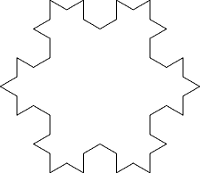
\includegraphics[]{koch.png}
  \caption{Koch curve drawn using turtle graphics}
  \label{fig:koch}
\end{figure}

\subsection{Lindenmayer Systems}

\begin{figure}[h!]
  \centering
  
\includegraphics[]{dragon.png}
  \caption{Dragon curve}
  \label{fig:dragon}
\end{figure}

L-Systems use formal grammar techniques to extend the possibilities of turtle graphics in a way fractals are easier producible. 

An L-system always consists of:
\begin{enumerate}
\item an alphabet $\mathcal{A}$, wich represents all the possible symbols in the generated string,
\item a dictionary $\mathcal{B}$, that maps every symbol from $\mathcal{A}$ to an action for the turtle graphics,
\item an axiom, a string in $\mathcal{A}$ that represents iteration zero,
\item an angle $\sigma$, the default angle for turning,
\item a set of production rules $X \rightarrow Y$, where $X$ is a character in $\mathcal{A}$ and $Y$ a string in $\mathcal{A}$
\end{enumerate}

Except for fractals, L-systems are very often used to generate plants and trees. The Koch curve in figure \ref{fig:koch} can be given as an L-system.

\begin{table}
\center
\begin{tabular}{l l}
Axiom & $F--F--F$ \\ \hline
$\sigma$ & 60\degree \\ \hline
Rules & $F \rightarrow F+F--F+F$ \\
\end{tabular}
\caption{The Koch-curve as an L-System}
\end{table}

\begin{figure}[h]
  \centering
  \subfloat[][Axiom]{\label{fig:koch1}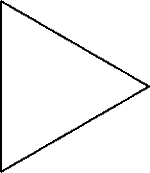
\includegraphics[width=0.23\textwidth]{koch1.png}}
  \hspace{0.01\textwidth}
  \subfloat[][First Iteration]{\label{fig:koch2}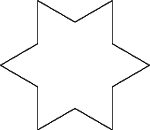
\includegraphics[width=0.23\textwidth]{koch2.png}}
  \hspace{0.01\textwidth}
  \subfloat[][Second Iteration]{\label{fig:koch3}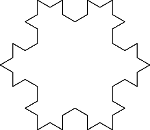
\includegraphics[width=0.23\textwidth]{koch3.png}}
  \hspace{0.01\textwidth}
  \subfloat[][Third Iteration]{\label{fig:koch4}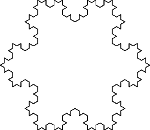
\includegraphics[width=0.23\textwidth]{koch4.png}}
  \caption{Iterating the Koch curve}
  \label{fig:animals}
\end{figure}

The power of an L-system is the way they generate strings using symmetries, fractals and flowers can be represented as very small files (usually under 1KB) but iterating them can produce complex images. To generate this complex images, the L-system must be iterated.
The axiom is iteration zero, it specifies the starting string. Iterating an L-system only once will replace every character in the string with the body of the respctively production rule. The second iteration will take the output of the first iteration and will replace these characters by there production bodies. For example, given an axiom $F--F--F$ and only one production rule $F \rightarrow F+F--F+F$ will produce the following output strings:
\begin{table}[h!]
\center
\begin{tabular}{l l}
Iteration & String \\ \hline \vspace{5pt}
0 \footnotesize (axiom) & $F--F--F$ \\ \vspace{5pt}
1 & $\underline{F+F--F+F}--\underline{F+F--F+F}--\underline{F+F--F+F}$ \\
2 & \footnotesize $\underline{\underline{F+F--F+F}+\underline{F+F--F+F}--\underline{F+F--F+F}+\underline{F+F--F+F}}--$ \\
  & \footnotesize $\underline{\underline{F+F--F+F}+\underline{F+F--F+F}--\underline{F+F--F+F}+\underline{F+F--F+F}}--$ \\
  & \footnotesize $\underline{\underline{F+F--F+F}+\underline{F+F--F+F}--\underline{F+F--F+F}+\underline{F+F--F+F}}$ \\
\end{tabular}
\caption{Generating the Koch curve}
\end{table}

\subsection{Extensions}
Although this basic set of commands allows us to draw some nice pictures, many extensions have been added to maximize the possibilities of L-Systems. The implemented extensions are given in this subsection.

\subsubsection{Brackets}
Brackets are used to save the current state (at least the current position and direction) to a stack. This allows us to start a subexpression as new branch, but return later on to the original position and continue its root branch.

\begin{center}
\begin{tabular}{c | l}
Symbol & Action \\ \hline
[ & Push the current state to the stack \\
] & Pop the last saved state from the stack \\
\end{tabular}
\end{center}

\begin{figure}[htb]
  \centering
  \begin{minipage}[c]{0.65\textwidth}
    \centering
    \begin{tabular}{l l}
Axiom & $X$ \\ \hline
$\sigma$ & $22.5$\degree \\ \hline
Rules & $X \rightarrow F-[[X]+X]+F[+FX]-X$ \\
& $F \rightarrow FF$ \\
	\end{tabular}
  \end{minipage}
  \begin{minipage}[c]{0.33\textwidth}
    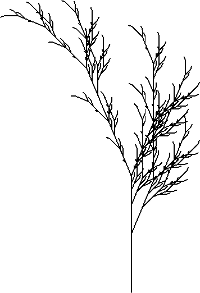
\includegraphics[width=\textwidth]{tree.png}
  \end{minipage}
  \caption{Simple 2D plant with brackets}
  \label{fig:tree}
\end{figure}

\subsubsection{3D}
To create more realistic models of objects, 3D was introduced. Instead of just turning left and right, it gives support for rotating the pen and adjusting its pitch.

\begin{center}
\begin{tabular}{c | l}
Symbol & Action \\ \hline
\& & Pitch down \\
\^{} & Pitch up \\
/ & Roll right \\
$\backslash$ & Roll left \\
$\vert$  & Turn 180\degree \\
\end{tabular}
\end{center}

\begin{figure}[htb]
  \centering
  \begin{minipage}[c]{0.65\textwidth}
    \centering
    \begin{tabular}{l l}
Axiom & $F$ \\ \hline
$\sigma$ & $28$\degree \\ \hline
Rules & $F \rightarrow F[\&+F]F[-\backslash F][\&F]$
	\end{tabular}
  \end{minipage}
  \begin{minipage}[c]{0.25\textwidth}
    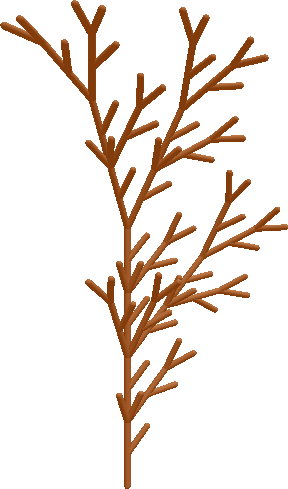
\includegraphics[width=\textwidth]{3dtree.png}
  \end{minipage}
  \caption{A 3D plant}
  \label{fig:3dtree}
\end{figure}

\subsubsection{Polygons}
To improve the realism of the models even more, flowers and leaves can be added to them. Therefore the drawing system should support polygons. The start of a polygons implies storing the position on the stack. When a polygon is started, for every position the pen moves to a new triangle will be created. This triangle is defined by three corners, the new position, the previous position, and the start position of the polygon. Obviously, after the first movement the startposition and the previous position are the same so no triangle can be created. To support this settings the state of the pen must be extended with a polygon mode, which must be set to true when we want to start a new polygon.
Figure \ref{fig:polygon} is the visualization of the following string ($\sigma = 30\degree$):
\begin{verbatim}
F{-f+f+f-|-f+f+f}
\end{verbatim}

\begin{figure}[h!]
  \centering
  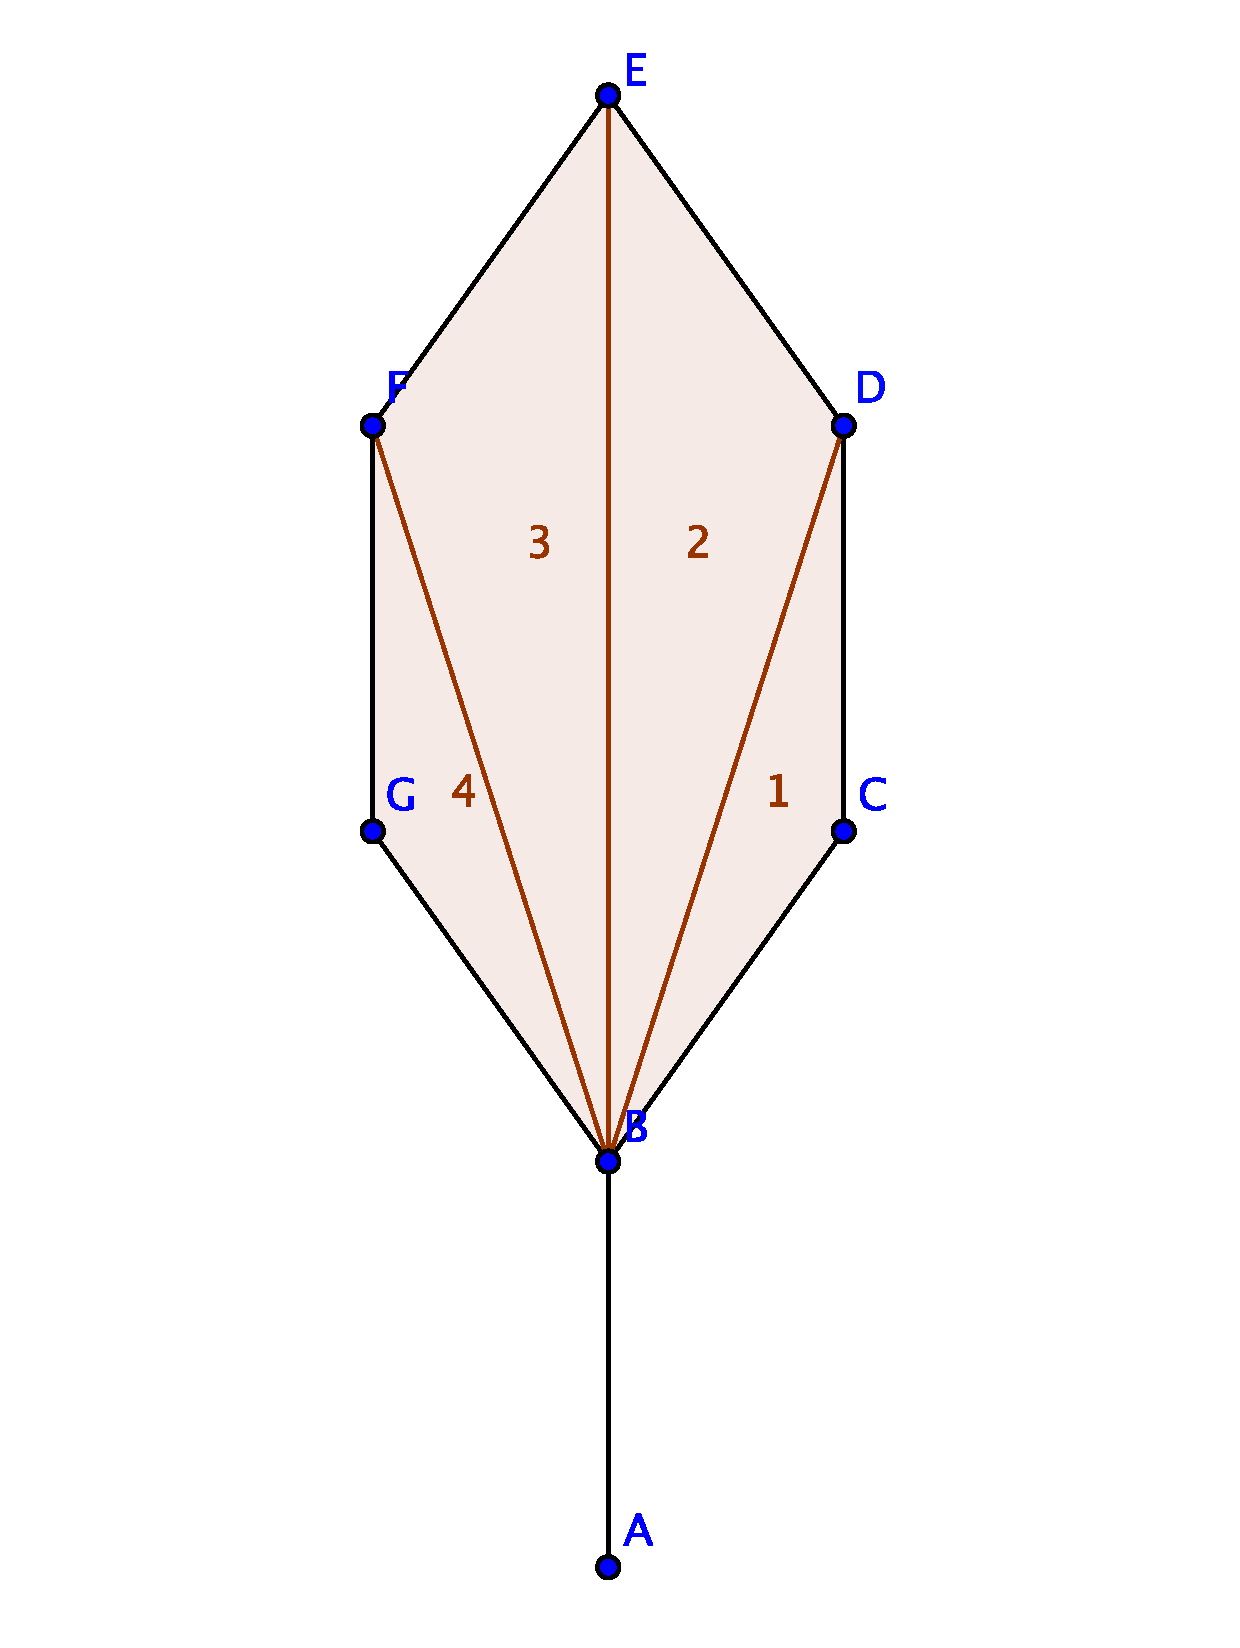
\includegraphics[width=0.35\textwidth]{polygons.pdf}
  \caption{How a polygon is drawn}
  \label{fig:polygon}
\end{figure}

\begin{center}
\begin{tabular}{c | l}
Symbol & Action \\ \hline
\{ & Push the current state to the stack and set polygon mode \\
\} & Pop the last saved state from the stack \\
\end{tabular}
\end{center}

\subsubsection{Pen style}
Another extension is the pen style, this includes both line length and thickness as the color. Default, an L-System starts with a line length of 1 and 10\% of the length as thickness. This allows us to draw a thick trunk and smaller branches, or brown trees with green leaves. The pen style is also part of the state, so it gets saved whenever we push the stack.

\begin{center}
\begin{tabular}{c | l}
Symbol & Action \\ \hline
! & Reduce thickness by 30\% \\
? & Increase thickness by 40\% \\
' & Reduce length by 10\% \\
" & Increase length by 10\% \\
c & Increase color index by 1
\end{tabular}
\end{center}


\subsubsection{Parameters}
The last implemented extension is the ability to give each command and optional parameter, specified between brackets after the command it applies to. Using parameters makes it possible to turn by an angle, other than $\sigma$ or specify a fixed color constant.

\begin{figure}[h!]
  \centering
  \subfloat[][Lily]{\label{fig:lilypov}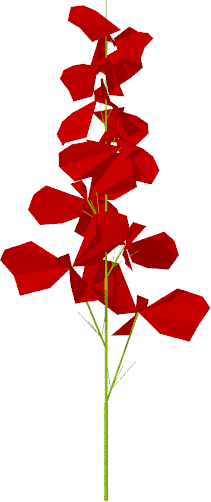
\includegraphics[width=0.27\textwidth]{lily_red.png}}                
  \subfloat[][Plant]{\label{fig:treepov}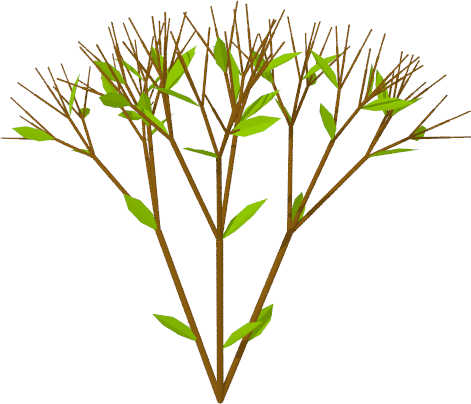
\includegraphics[width=0.73\textwidth]{plant6.png}}
  \caption{POVRay renders of L-Systems}
  \label{fig:povrenders}
\end{figure}

\begin{center}
\begin{longtable}{l | l}
Symbol & Action \\ \hline
F & Draw a line of 1 unit \\
F(x) & Draw a line of x units \\
f & Move forward by 1 unit \\
f(x) & Move forward by x units \\
Z & Draw a line of half a unit \\
Z (x) & Draw a line x/2 units \\
z & Move half a unit \\
z(x) & Move by x/2 units \\
+ & Turn left over $\sigma$ \\
+(x) & Turn left over x\degree \\
- & Turn right over $\sigma$ \\
-(x) & Turn right over x\degree \\
$[$ & Push the current state to the stack \\
$]$ & Pop the last saved state from the stack \\
\& & Pitch down over $\sigma$ \\
\&(x) & Pitch down over x\degree \\
\^{} & Pitch up over $\sigma$ \\
\^{}(x) & Pitch up over x\degree \\
/ & Roll right over $\sigma$ \\
/(x) & Roll right over x\degree \\
$\backslash$ & Roll left over $\sigma$ \\
$\backslash$(x) & Roll left over x\degree \\
$\vert$  & Turn 180\degree \\
\{ & Push the current state to the stack and set polygon mode \\
\} & Pop the last saved state from the stack \\
! & Reduce thickness by 30\% \\
? & Increase thickness by 40\% \\
!(x),?(x) & Thickness = thickness * x \\
' & Reduce length by 10\% \\
" & Increase length by 10\% \\
'(x),"(x) & Length = length * x \\
c & Increase color index by 1 \\
c(x) & Set color index to x \\
\end{longtable}
\end{center}

\subsection{Efficiency} % both time and space approach and complexity
Implementing a program to calculate and draw Lindenmayer systems is not a big challenge. There is a very naive way of doing this, which will be explained later on, but this method is in general very slow and consumes huge amounts of memory. We will try to speed things up by implementing a more complex data structure and using some general optimizations. The approach of this project was to minimize both time and space complexity.

\newpage
\section{Implementation}

A Lindenmayer system in a datastructure always consists of:
\begin{enumerate}
\item An alphabet \label{structalpha}
\item An axiom, a string \label{structaxiom}
\item A list of production rules, a pair (character, string) \label{structrules}
\item A default angle $\sigma$, a double for the radial of degree representation
\item A dictionary, telling what characters cause what action
\item Optionally a set of colors
\end{enumerate}
Only \ref{structalpha}, \ref{structaxiom} and \ref{structrules} are required for the string production. And since the alphabet is usually the machines character set, there is no need to store this in the program.

\subsection{String iteration, the naive approach}

Iterating L-systems is not very difficult using string iteration. Your program only needs the production rules and the axiom, no preprocessing is required. From the previous step or axiom, the program loops over every character and adds the substitution of that character to the new string or the character itself if no production rule is found.

\lstset{label=code:stringit,caption=String iteration}
\begin{lstlisting}
//Given: axiom (string), rules (array of string)
currentstring = axiom
iteration = 0

function iterate()
	newstring = ""
	iteration = iteration + 1
	foreach c in currentstring
		if (c in rules)
			newstring = newstring + rules[c]
		else
			newstring = newstring + c
	currentstring = newstring
\end{lstlisting}

The code \ref{code:stringit} shows the algorithm to iterate currentstring to the next iteration. This is a fairly easy implementation of both the algorithm and the datastructure but has some huge disadvantages: iterating the L-system found in \ref{fig:3dtree} only 12 times returns a string of size 915527344 (~873 MB). Besides the memory usage, it took tens of minutes to process the last 3 iterations. Another small disadvantage is the fact you cannot go back one iteration without recalculating it from the axiom to that iteration.

For the complexities, let $I$ be the iteration level, $n$ the average production body length, $s$ the total string length, $p$ the average number of replacement symbols in one production body or axiom and $p_t$ the total number of productions and the axiom.
The time complexity to build this structure is $O(p^I)$. When it is build, the time needed to request one character is $O(1)$, since an array allows direct memory access. This brings the total complexity to build the structure an traverse it once at $O(p^I)+s*O(1) = O(p^I+s)$.
The space complexity is $O(n^I)$. Both time and space complexity are non-polynomial, so we will try to improve this.

\subsection{A more efficient data structure} %and maybe the draw inside the calc

The only production rule in \ref{fig:3dtree} is $F \rightarrow F[\&+F]F[-\backslash F][\&F]$. So every F in the axiom will be replaced by the same string. The next iteration should only iterate that string once, and it will be correct for every occurence of F in the original string. This will speedup the iteration time and decrease the memory usage of the string representation drastically.


\begin{figure}[h!]
  \centering
  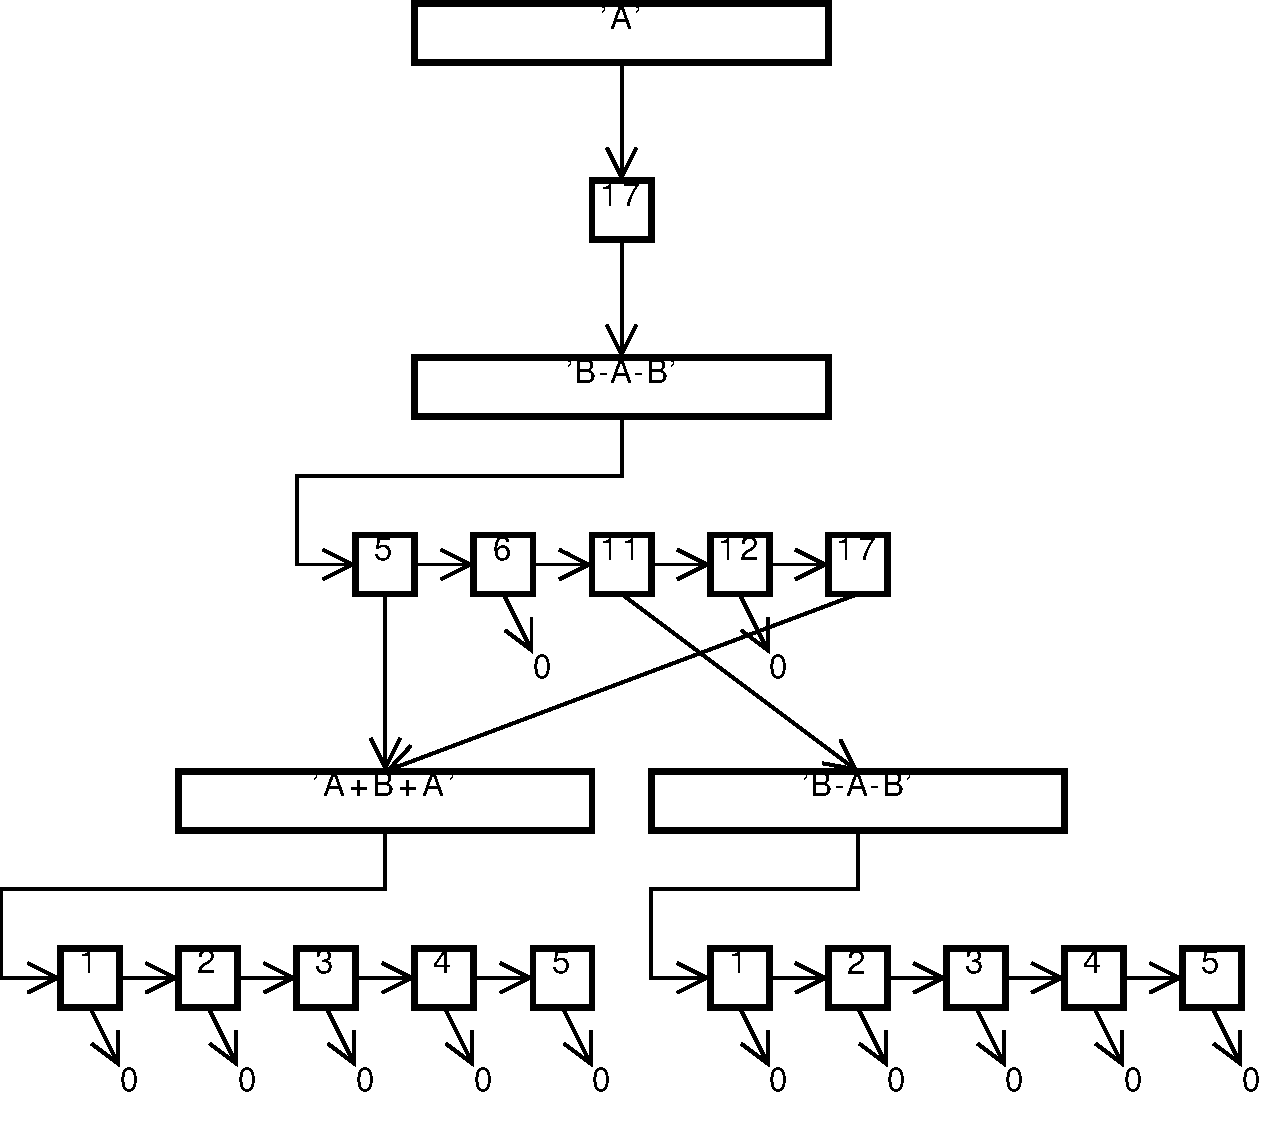
\includegraphics[width=0.9\textwidth]{struct.pdf}
  \caption{A tree based datastructure that represents the dragoncurve at level 2}
  \label{fig:struct}
\end{figure}

The string will be stored as a tree-like datastructure similar to the one in \ref{fig:struct}, with the axiom as root node. Each node consists of 2 arrays. A char array, wich is just the string representation of the node, and an array of pointers, wich point the replacement of the respectilely character at the next iteration level. If the character is a terminal (there exists no production body for this), its pointer will be null. If the iteration level is the last one calculated, the whole array will be null.

The nodes are kept by one common object that manages the creation and deletion of these nodes. This object will assure that no object will be created if it already exists for the requested iteration level.

Besides the two arrays in a node, a third array is stored in each node wich represents the total length of the whole string for every position of the substring. In a leaf node this array will be the sequence 1 to length, as no character will be replaced. In other nodes the step between 2 elements in this array is equal to the length of its childnode at the given position. Due to this sorted list, a binary search can be used to find wich childnode must be searched to find the character for a requested index.

When an iteration level gets deeper and the production bodies are small, every level must me visited to find the character of a corresponding index. To speed this up a buffer can be used in every node wich length of replaced string is less than a given threshold.

A small threshold will not reduce the number of steps needed to find a character very much, but a big threshold will store much more data in every node, so this threshold must be choosen carefully.

When drawing the string, it will be read from front to back, and for each character the tree must be traversed. Since most characters will be found in the same node as the previous request (certainly if using buffers) it is usefull to store some information about the last path. When requesting a character, the node that holds the character stores his position in a certain directpath pointer, and stores the number of characters left the same node. This information can be used as a direct path instead of traversing the whole tree.

\begin{table}
\center
\begin{tabular}{l l}
Axiom & $A$ \\ \hline
$\sigma$ & 90\degree \\ \hline
Rules & $A \rightarrow B-A-B$ \\
      & $B \rightarrow A+B+A$ \\
\end{tabular}
\caption{The L-system of the dragoncurve}
\end{table}

The time complexity to build this structure is much less, since at every iteration level, a spcific node must be calculated only once, and must be stored only once so it will bring down the space complexity as well.
Time complexity to build the structure is at worse $O(I*p_t)$.
Requesting one character in the structure will take $O(I*log(p))$ time, but due to the direct path pointer, requesting the whole string sequencally will take only $O(\frac{s}{n} * I*log(p) + (s-\frac{s}{n}) * 1)$ time. The first term are the number of full traversals needed times the traversal of the tree (the number of iterations times a binary search). The second term represents the number of direct accesses. This makes a total time complexity of $O(I*p_t + \frac{s}{n} * I*(log p) + (s-\frac{s}{n}) * 1) = O(I * (p_t + \frac{s}{n} * log(p)) + (s - \frac{s}{n}))$. If a buffer is used, $n$ can be replaced by the buffer size.
The space complexity for this structure is $O(I*p_t*n)$, wich is the number of iteration levels with at each level a node of size n for every production.

\subsection{Real life differences} %benchmark results

These benchmark result are dependent on the implementation details of the programs. The time column was only the building of the datastructure, not the traversal, so the tree based structure might benifit these results. The time was the average of 5 runs. 0 (not iterating) is included to give an impression of the preprocessing time and space.

\begin{table}
\center
\begin{tabular}{r r r r r}
Depth & N time & N memory & TB time & TB memory \\ \hline
0  & 0.006 s & 252.7 KB & 0.010 s & 384.7 KB \\ \hline
5  & 0.011 s & 253.6 KB & 0.011 s & 386.4 KB \\ \hline
10 & 0.012 s & 276.6 KB & 0.010 s & 390.3 KB \\ \hline
15 & 0.016 s & 758.0 KB & 0.010 s & 391.6 KB \\ \hline
20 & 0.176 s &  16.2 MB & 0.013 s & 393.0 KB \\ \hline
25 & 5.256 s & 512.2 MB & 0.010 s & 394.3 KB \\
\end{tabular}
\caption{Time and space in real life, N=Naive implementation, TB=Tree based implementation}
\end{table}

\begin{figure}[h!]
  \centering
  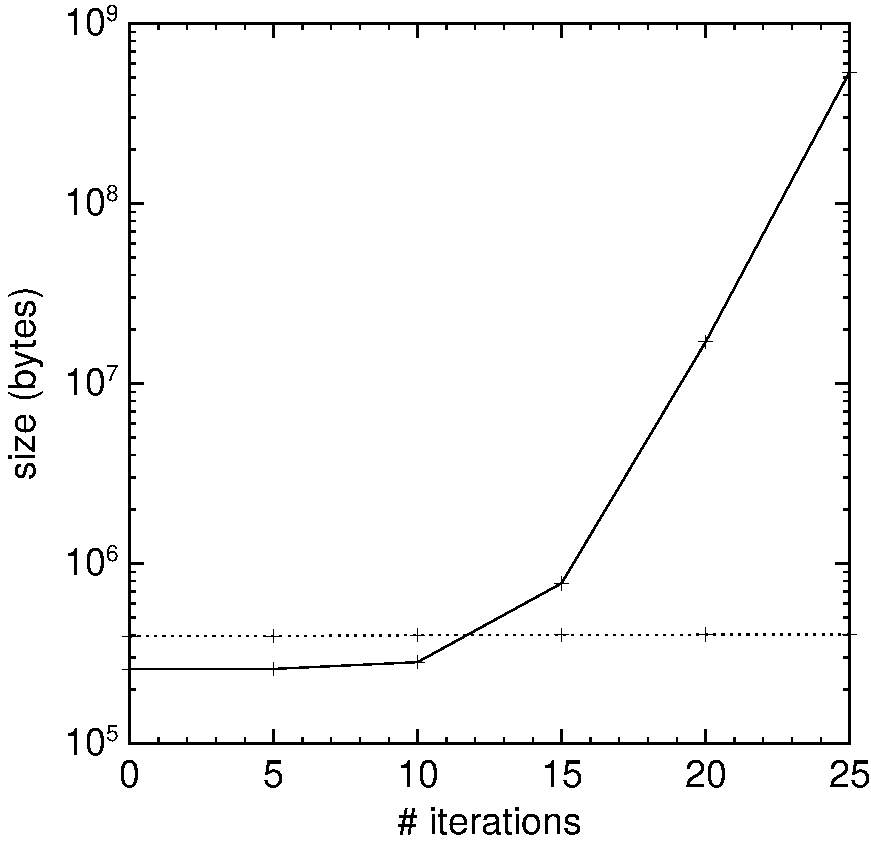
\includegraphics[width=0.8\textwidth]{bench.pdf}
  \caption{Memory usage for naieve approach (solid line) versus tree based strcuture (dotted line)}
  \label{fig:bench}
\end{figure}

\subsection{Calculating geometry}

When the string structure is built, the objects geometry must me calculated. For this, the string must be traversed from the beginning to the end, and for every character a transformation must be made. The shorter the string, the less processing time, so we can use compression techniques that don't make the string harder to process. Run-length encoding (RLE) is an example of a string compression technique that keeps the string easy processable. For example, the RLE algorithm will compress the string $+++++//////$ to $+`5/`6$, instead of just shortening the string, the processor will read $+`5$ as $+(sigma*5)$ and that will take up only one action. Furthermore, the LRE algorithm can be modified to compress strings like $+--++++$ to $+`3$ and $+++--+--$ to an empty string.
Another scenario that will slow down the processing speed are L-systems that contains production bodies with parameters. For example the production rule $X \rightarrow F(0.3333)+F(0.3333)--F(0.3333)+F(0.3333)$. Each time an F is encountered, the tail string will be tested for a parameter. When the test returns true, it must process the string to a double. This process is quite expensive and can be eliminated using an inlined parameter reference. This means every production and the axiom will be preprocessed. In this inline process, every parameter encountered will be pushed in a vector and a reference to the vector index will replace the parameter in the string. The production body of the given example after preprocessing it might look like $F\tilde{ } 1+F\tilde{ } 1-`2F\tilde{ } 1+F\tilde{ } 1$ and a vector $p[1]=0.3333$. Not only is this rewritten body shorter so needs less storage space, it will also be processed faster, since the parameter (0.3333) doesn't have to be converted from string to double everytime it is encountered.
These preprocessing technique shortens the processing time of a string by $\pm 30\%$.

\subsection{Improving the efficiency}

% a histogram for compiler options benchmarking?

\section{Stochastic L-Systems} %and how it fucks the datastructure
\subsection{Implementation}



\subsection{Memory usage}


\section{Conclusion}

\newpage
\begin{appendix}
\listoffigures
\end{appendix}
\end{document}